% LaTeX Article Template - customizing header and footer
\documentclass{article}

\newtheorem{thm}{Theorem}

% Set left margin - The default is 1 inch, so the following 
% command sets a 1.25-inch left margin.
\setlength{\oddsidemargin}{0.25in}

% Set width of the text - What is left will be the right margin.
% In this case, right margin is 8.5in - 1.25in - 6in = 1.25in.
\setlength{\textwidth}{6in}


% Set top margin - The default is 1 inch, so the following 
% command sets a 0.75-inch top margin.
\setlength{\topmargin}{-0.25in}

% Set height of the header
\setlength{\headheight}{0.3in}

% Set vertical distance between the header and the text
\setlength{\headsep}{0.2in}

% Set height of the text
\setlength{\textheight}{9in}

% Set vertical distance between the text and the
% bottom of footer
% Set the beginning of a LaTeX document
\usepackage{multirow}
\usepackage{fullpage}
\usepackage{graphicx}
\usepackage{amsthm}
\usepackage{amssymb}
\usepackage{algpseudocode}
\usepackage{tikz-qtree}
\usepackage{qtree}
\usepackage{amsmath}



\graphicspath{ {images/} }


\begin{document}\title{CSCI-B657 \\Assignment 2: Image Warping, Matching and Stitching Basics}         % Enter your title between curly braces
	\author{Prakash Rajagopal \\ Sagar Bhandare \\ Suhas Jagadish\\ }        % Enter your name between curly braces
	\date{\today}          % Enter your date or \today between curly braces
	\maketitle
	
	\makeatother
	
	\pagestyle{plain}
	\begin{enumerate}
		\item Write a function that takes two images, applies SIFT on each one, finds matching SIFT descriptors across the two images, and creates an image. 
		
		Solution: The steps taken to perform the above task are - \newline
		- First step is to convert both the query image and target image to grayscale. \newline
		- Sift descriptors are then computed for both the grayscale images.\newline
		- We then iterate over all the descriptor values of the target image for each value of query image to find the minimum euclidean distance. \newline
		- The closest and second-closest match is computed. If the ratio of closest to second-closest is less than the threshold, then we treat the point as the best point. All the best points are stored in a vector. \newline
		- The query and target images are merged together and a yellow line is drawn between the matching points. \newline
		The result of above steps is depicted in the below image, considering "bigben\_2" as query image and "bigben\_3" as target image - 
		
		\begin{center}
			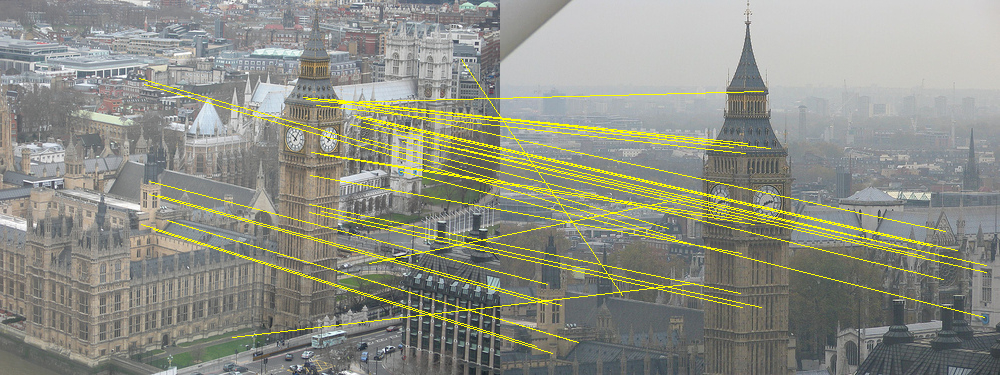
\includegraphics[width=16cm, height=8cm]{result_sift_match.jpg} \\
		\end{center}
		
		\item Use your functions above to implement a simple image retrieval program, that searches an image library to find the best matches for any given query image. The program should then output the list of remaining images, sorted in decreasing order of number of matched features. 
		
		Solution: The steps taken to perform the above task are - \newline
		- The query image is run against a set of target images. \newline
		- All the target images are stored in a vector called "compare\_images". Then for each image in this vector, we calculate the sift descriptors and match the key points with our query image using the technique described in problem 1. \newline
		- A priority queue can be used in this scenario where the top of the queue always contains the greatest element. We pass the number of matching points for the comparator and everytime we insert a new matching point value, it ensures that the one with the highest number of matching points stays at the top. \newline
		- All the image names are displayed starting from the top of the queue which gives us the list of target images, sorted in decreasing order of number of matched features.
			\begin{center}
				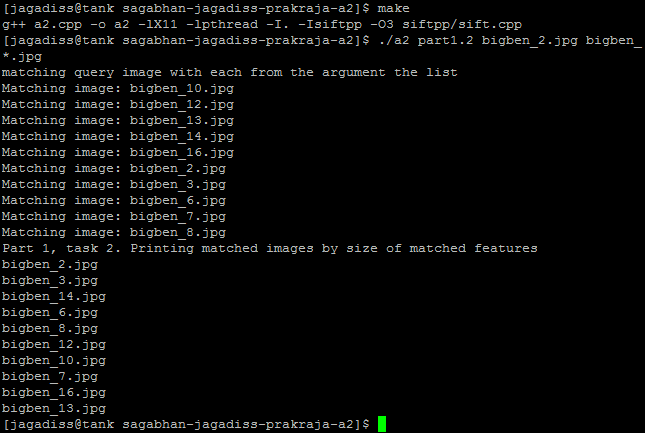
\includegraphics[width=10cm, height=7cm]{p1-q2.png} \\
			\end{center}
		
		\item To measure the performance of your retrieval algorithm on this task, conduct the following experiment. For each of the 10 attractions, choose 1 image of that attraction at random to use as the query image, and then pass all 100 images as the others. Look at the top 10 ranked images returned by your program, and calculate the percentage
		of images that are from the correct attraction. This is called the precision of your system. Repeat this	process for each of the remaining attractions, and present the results in your report. Which attractions seem to be the easiest to recognize, and which are most difficult? 
		
		Solution: The steps taken to perform the above task are - \newline
		- The directory containing all the 100 images and the query image are passed as arguments. \newline
		- Function "get\_files" lists all the files in the specified directory and the result is stored in a vector. \newline
		- Sift descriptors are calculated for each image in the vector and key points are matched with our query image using the technique described in problem 1. \newline
		- For the top 10 ranked images, we calculate the precision by matching the filenames of the query image and matched image. \newline
		- The above step is repeated for each of the 10 attractions and the results are tabulated. \newline
		- One thing to notice in this problem is that, accuracies of each attractions varied as we varied the threshold. We tried to vary the threshold for each of the 100 images to yield the best precision. Plots of threshold vs accuracy for each of the best picked 10 attractions is depicted below. \newline
		- The results are then tabulated with best accuracy for each of the 10 attractions as represented in Table 1. \newline
 
		
		\begin{figure}
			\fbox{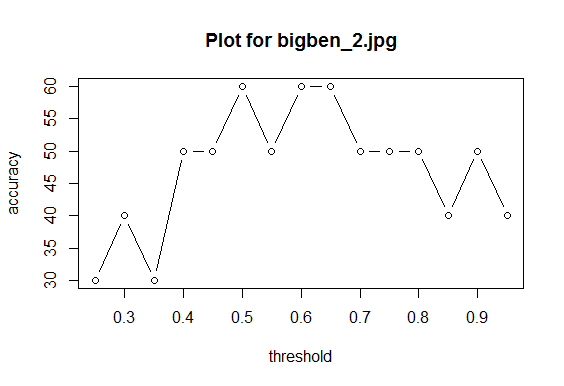
\includegraphics[width=4cm, height=3cm]{bigben.png}}   
			\hspace{10px}
			\fbox{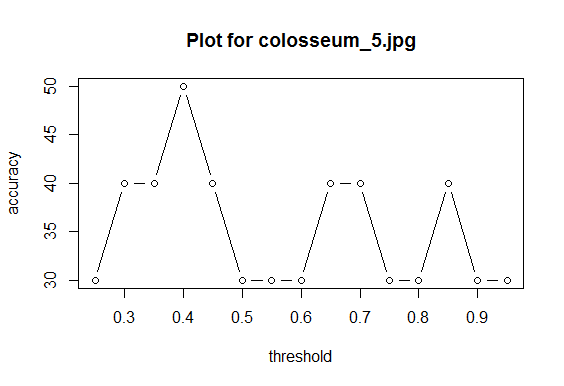
\includegraphics[width=4cm, height=3cm]{colosseum.png}}   
			\hspace{10px}
			\fbox{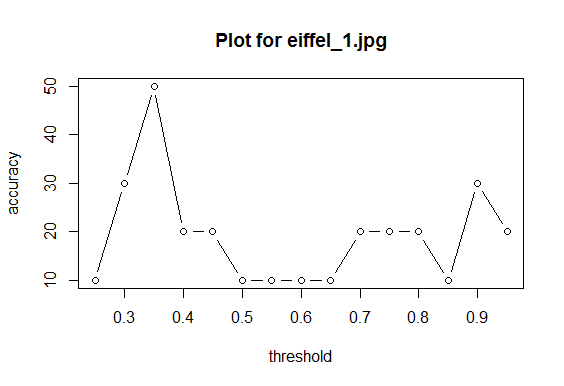
\includegraphics[width=4cm, height=3cm]{eiffel.png}}   
			\hspace{10px}
			\fbox{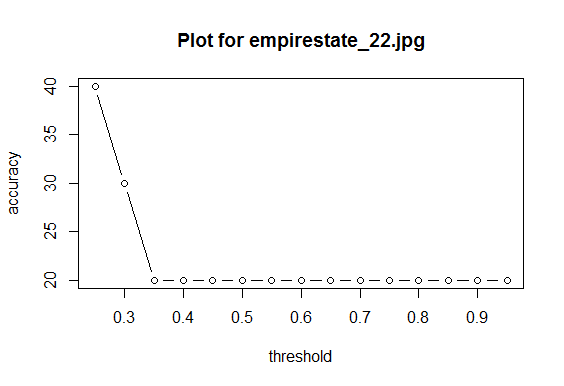
\includegraphics[width=4cm, height=3cm]{empirestate.png}}   
			\hspace{10px}
						\fbox{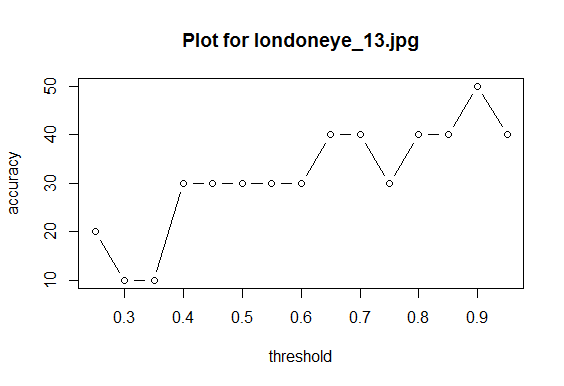
\includegraphics[width=4cm, height=3cm]{londoneye.png}}   
						\hspace{10px}
						\fbox{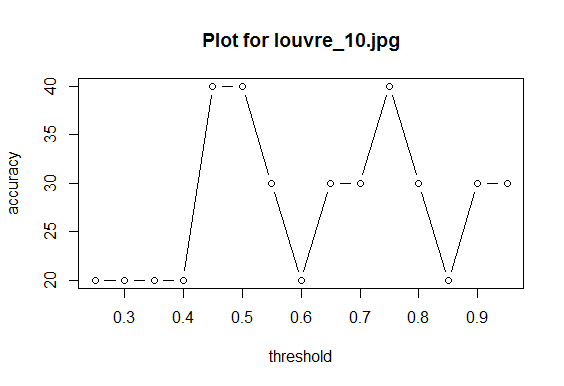
\includegraphics[width=4cm, height=3cm]{louvre.png}}   
						\hspace{10px}
						\fbox{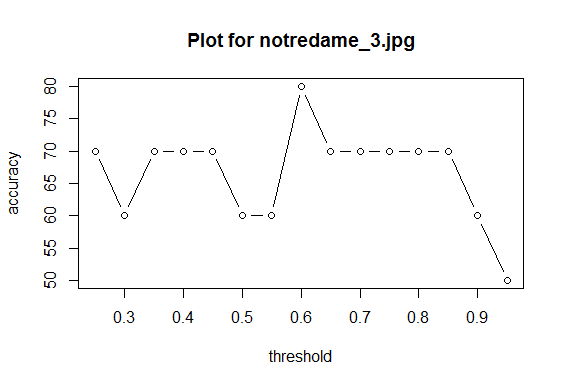
\includegraphics[width=4cm, height=3cm]{notredame.png}}   
						\hspace{10px}
						\fbox{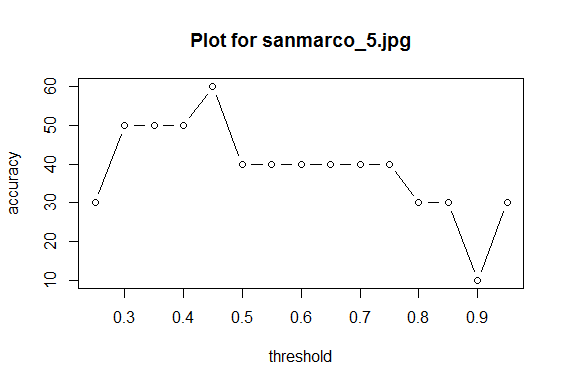
\includegraphics[width=4cm, height=3cm]{sanmarco.png}}   
						\hspace{10px}
					\fbox{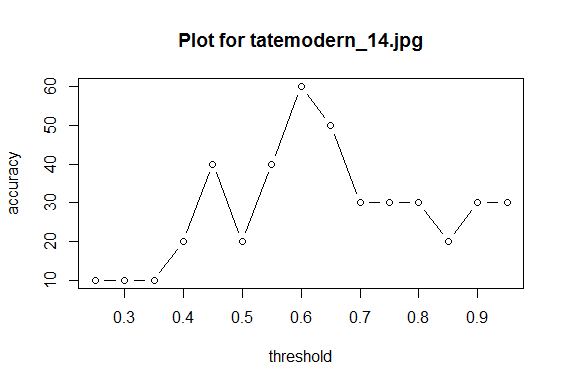
\includegraphics[width=4cm, height=3cm]{tatemodern.png}}   
					\hspace{10px}
					\fbox{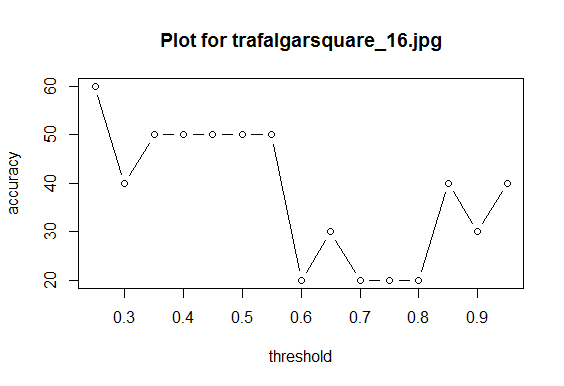
\includegraphics[width=4cm, height=3cm]{trafalgarsquare.png}}   
					\hspace{10px}
		\end{figure}
		
		\begin{table}[!htbp] \centering 
			\caption{Results of precision} 
			\label{} 
			\begin{tabular}{@{\extracolsep{5pt}} cccc} 
				\\[-1.8ex]\hline 
				\hline \\[-1.8ex] 
				& Attractions & Threshold & Accuracy \\ 
				\hline \\[-1.8ex] 
				1 & bigben\_2.jpg & $0.500$ & 60\% \\ 
				2 & colosseum\_5.jpg & $0.400$ & 50\% \\ 
				3 & eiffel\_1.jpg & $0.350$ & 50\% \\ 
				4 & empirestate\_22.jpg & $0.250$ & 40\% \\ 
				5 & londoneye\_13.jpg & $0.900$ & 50\% \\ 
				6 & louvre\_10.jpg & $0.500$ & 40\% \\ 
				7 & notredame\_3.jpg & $0.600$ & 80\% \\ 
				8 & sanmarco\_5.jpg & $0.450$ & 60\% \\ 
				9 & tatemodern\_14.jpg & $0.600$ & 60\% \\ 
				10 & trafalgarsquare\_16.jpg & $0.250$ & 60\% \\ 
				\hline \\[-1.8ex] 
			\end{tabular} 
		\end{table}
		
				- Number of distinct or unique features in a image is an important factor while comparing two images. If we look at "bigben", "notredame" and "tatemodern", they all have lot of matching points because they have many distinct features and all the images are clicked from somewhat similar projection. Hence they are quiet easy to recognize. But images such as "louvre" and "colosseum" have pictures taken from different angles, pictures with outer and inner layers and relatively less distinct points to match. Hence we found these little difficult to recognize.

		\item Implement the quantized projection function for the image matching. Does the algorithm speed up image retrieval, and if so, by how much? Does the approximation seem to affect the quality of results? Give quantitative answers to these questions if possible. What is the best trade-off you can achieve between running	time and accuracy, by adjusting w, k, and the number of trials?
		
		Solution: The steps taken to perform the above task are - \newline
		- Finalize value of K (reduced dimensions), W (step size) and generate K sample vectors of size 128 each from uniform distribution of variable x between [0,1].\newline
		- For all the descriptors of two images, img1 and img2 calculate summary vectors by taking dot product of sift descriptor with sample vectors.\newline
		- This step takes time O(m + n) where m and n denotes number of key-points in img1 and img2.\newline
		- Now, compare both newly generated summary vectors for each summary vector in img1 to find similar summary vectors in img2. Keep top 3 matches with least distance.\newline
		- This step takes time O(m*n*k).\newline
		- From top 3 matches calculate actual distance using euclidean distance function and pick key-point with least distance as best match.\newline
		- Repeat this process multiple time and choose most occurring point.\newline
		Observations:\newline
		- The algorithm does speed up the image retrieval. The speed up is proportional to the size of K chosen. It changes time complexity from m*n*128 to m*n*k. Figure k-time plots K vs Time required values. The speed up is almost linear.\newline
		- The reduced execution time comes with cost of quality of answer. With increased value of K the accuracy increases. Being said this there is no linear relation between value of k and accuracy as there is some randomness involved. Typically small and high values of K has given better values. We got accuracy above 50% with k < 10 and k > 40. 
		- We performed series of experiment to understand the trade off between k,w, and number of trials. The results are plotted in the graphs displayed at the top of the page. \newline \newline
	\begin{figure}
			\fbox{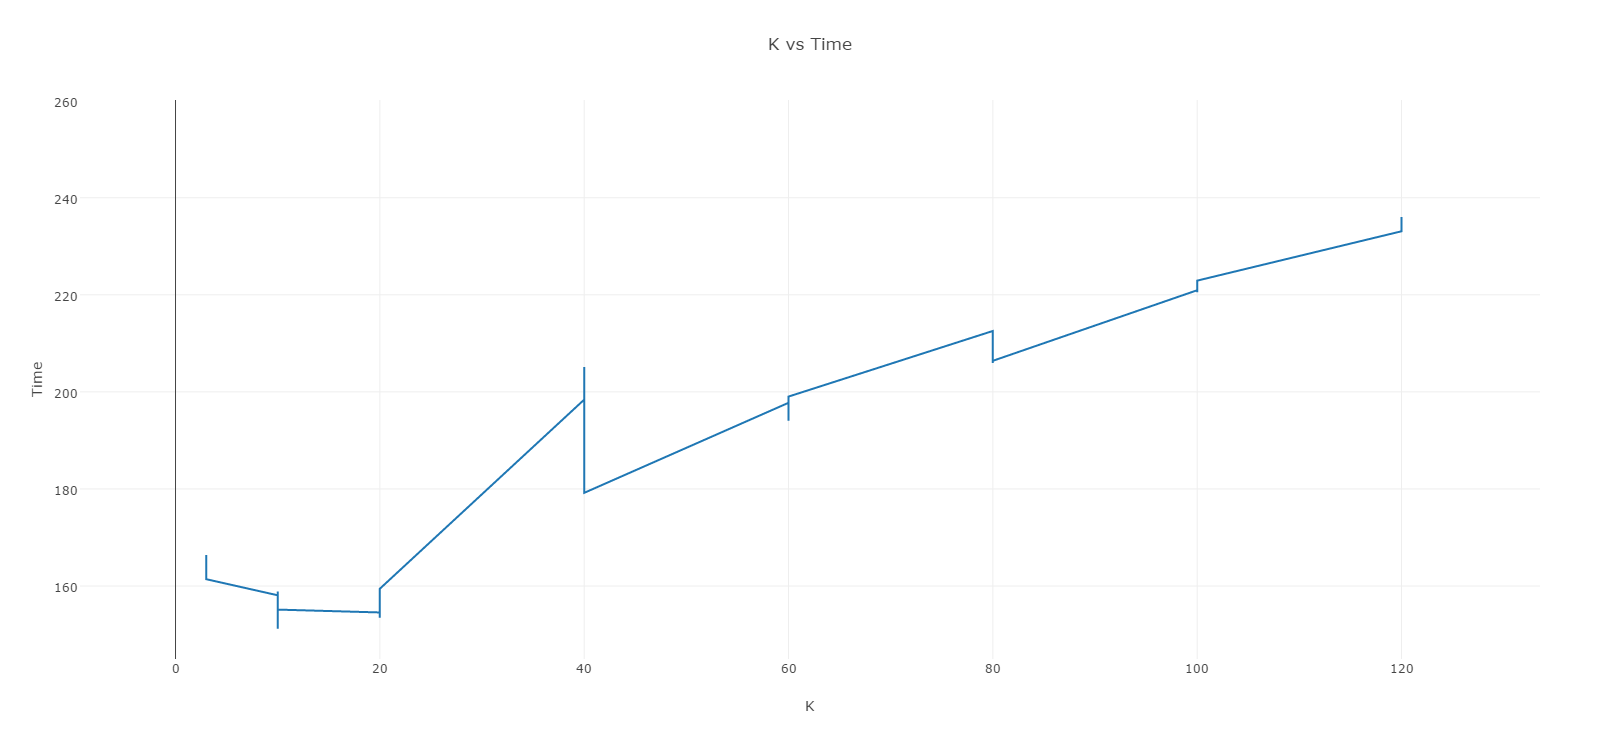
\includegraphics[width=5cm, height=3cm]{k-time.png}}   
			\hspace{15px}
			\fbox{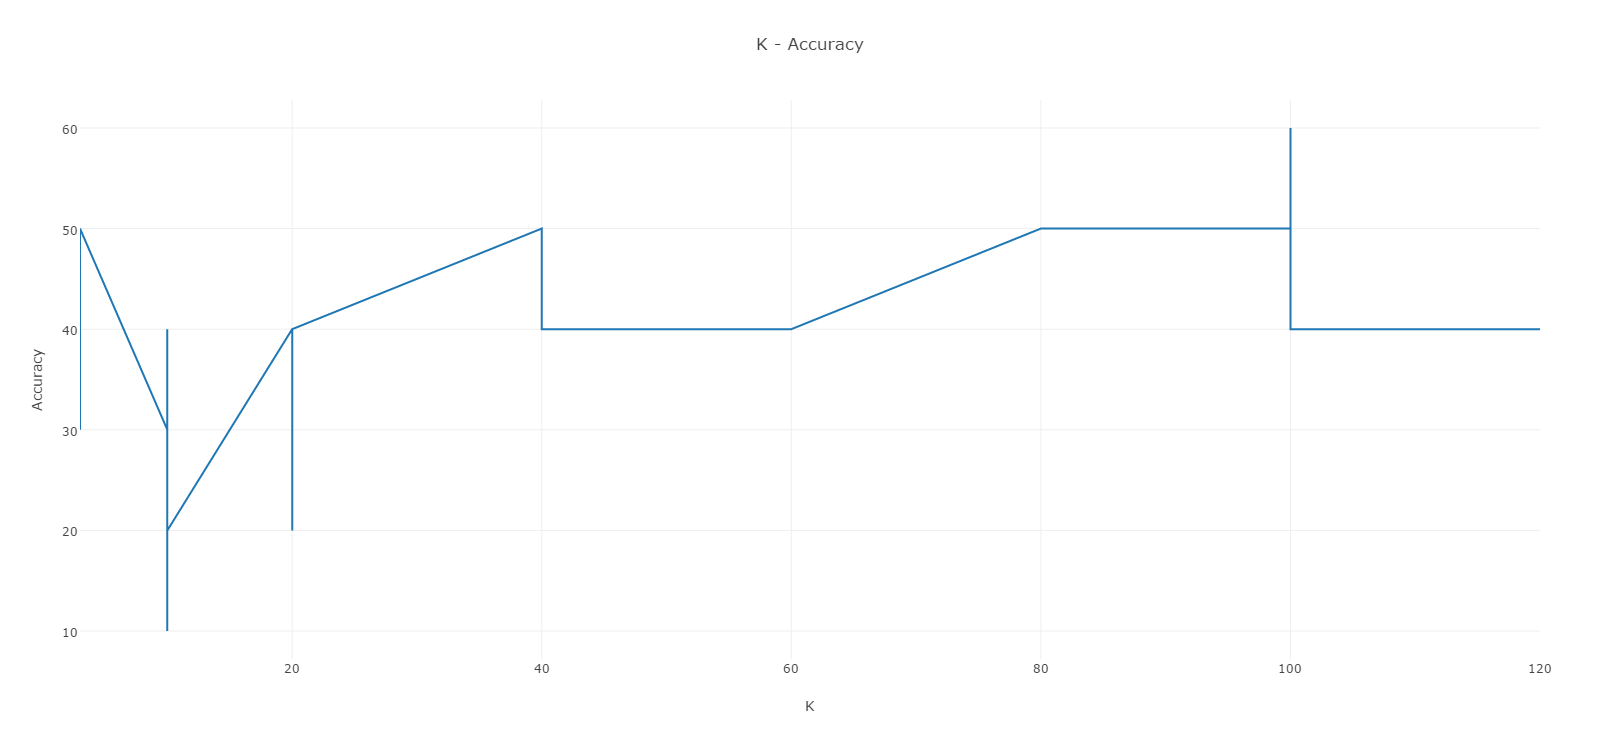
\includegraphics[width=5cm, height=3cm]{k-acc.png}}   
			\hspace{15px}
			\fbox{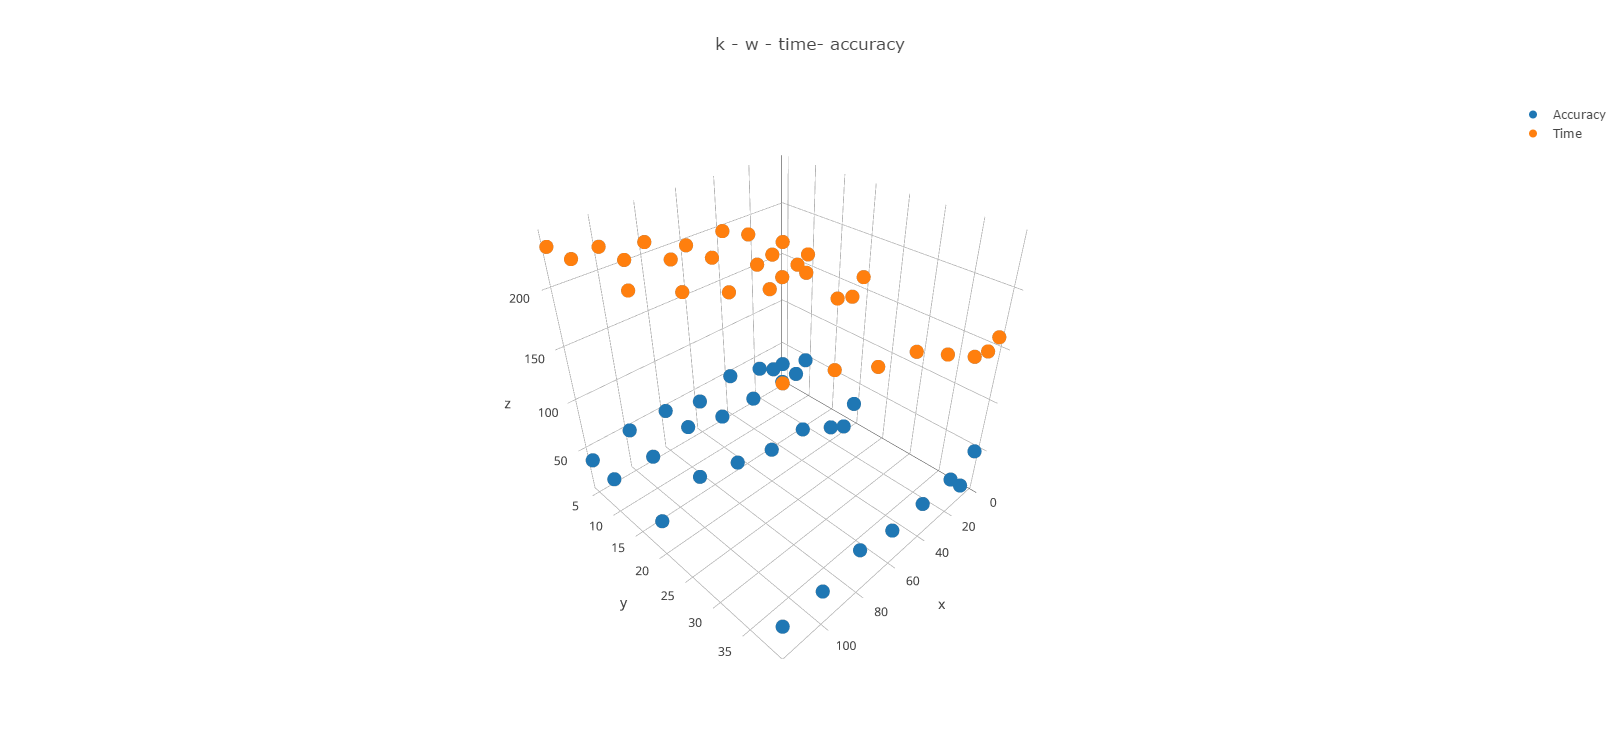
\includegraphics[width=5cm, height=3cm]{k-w-t-a.png}}   
		\end{figure}
		Trade off:\newline
		- Number of trails increase the time required of execution by considerable amount with not much gain in accuracy. However changing values of k and W gives considerable increase in accuracy.\newline
		- The best results are obtained at K = 100, W = 20. However K = 3 and W = 10 will give better results in very time efficient way.	\newline

	Additional efforts:\newline
	- Along with the tasks given in the homework we performed many additional tasks, tried various new ideas, analyzed program in various ways. I am describing one of the ideas that we worked on and implemented code for. We tried to develop better sift matcher which will not only consider the ratio between the top best matches but also considers the homography of matches.\newline
	- Following is the proposed and implemented algorithm for optimized sift matcher\newline
	- For two images img1 and img2, to be matched, calculate sift descriptors.\newline
	- Set very low threshold of 0.3 for the ratio between top 2 best matches.\newline
	- Match the two descriptors using euclidean as distance function till there are at least 30 matches, if not increase the threshold by 0.05 and repeat above steps.\newline
	- After getting 30 match points, apply RANSAC algorithm to calculate homography matrix. This will be approximate matrix.\newline
	- Restart the matching process of sift descriptors with newly generated homography matrix. \newline
	- Match each key-point descriptor to all the key-points of other image using euclidean distance and store results in priority queue.\newline
	- Remove top ten matches from the queue.\newline
	- Select a match having ratio less than threshold with its successor and matching the projected co-ordinates by homography matrix with tolerance of 20px.\newline
	- This algorithm provides a better sift matches than normal algorithm with euclidean as distance function.\newline
		\end{enumerate}
		
	
	Part 2: Image warping and homographies
	\begin{enumerate}
		\item Write a function that takes an input image and applies a given 3x3 coordinate transformation matrix (using homogeneous coordinates) to produce a corresponding warped image.
		
		Solution: The steps taken to perform the above task are - \newline
		- An input image is chosen and a projective transform is applied to the image using the given matrix. \newline
		- The function uses inversion technique. It takes the inverse of the matrix and then for each pixel in the new image, it calculates its corresponding position in the original image. \newline
		- The transformed output is created in a file called "res.png". 
		\begin{center}
			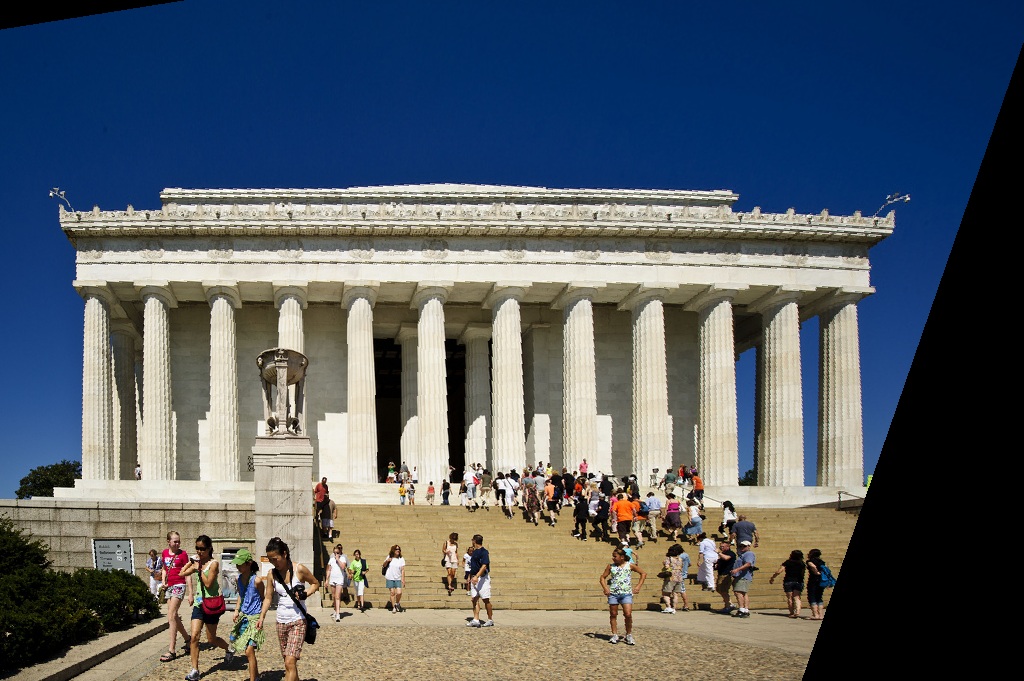
\includegraphics[width=16cm, height=8cm]{res.png} \\
		\end{center}
		
		\item Write a function that automatically estimates a homography (projective transformation) between two images. Implement this using RANSAC, as we discussed
		in class. 
		
		Solution: Given a set of images, our function calculates the projection matrix and prints it at first. \newline
		- SIFT matching is then applied to get a set of matching points. \newline
		- RANSAC is implemented to compute the matrix. The algorithm basically calculates the projective matrix using a set of 4 random points and then compares the quality of the result by checking if the match source corresponds to correct destination using this matrix. \newline
		- The function takes the best computed result after 100 rounds. \newline
		- This creates a warped image that is required in 2.3. 
		
		\item Combine your homography estimation and your warping code to create an image sequence warping application.
		
		Solution: This is similar to the previous problem but run with multiple files. \newline
		- The function uses the matrix from the previous step and transforms the second image using that matrix. It then writes to <file>\_warped.jpg with an image which is in the same camera angle as the source image. \newline
		- The results displayed in the next page shows the original image, input image 1 and its warped image, input image 2 and its warped image in 3 successive rows. The warped images appears to have been taken in the original image's camera's coordinate system.
		\newline 
		 
		\begin{figure}
		\fbox{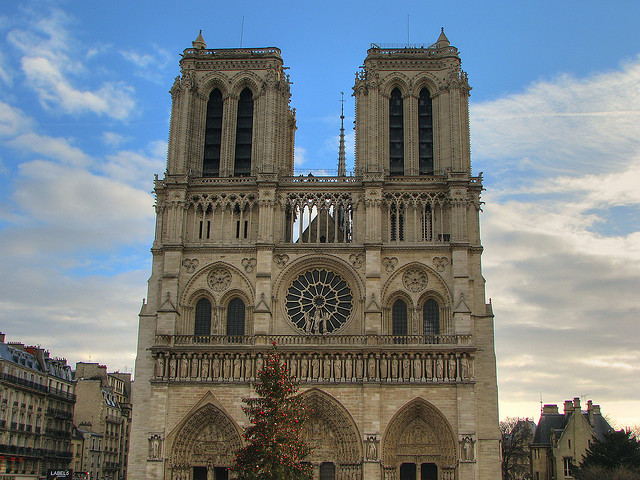
\includegraphics[width=10cm, height=8cm]{2298146191_888de5b755_z_d.jpg}} \\
		 Original image \newline \newline \newline
		\fbox{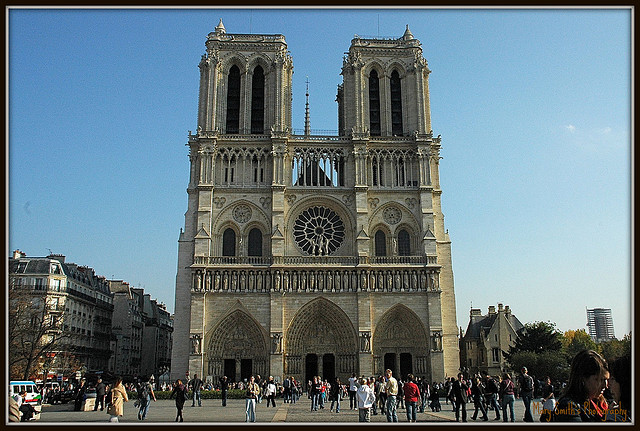
\includegraphics[width=8cm, height=6cm]{3268706748_0d2c67f3c3_z_d.jpg}} 
		\hspace{20px}
		\fbox{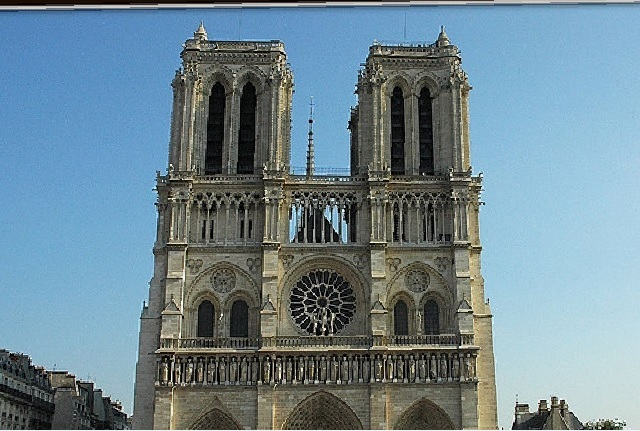
\includegraphics[width=8cm, height=6cm]{image1-warped.jpg}}
		\hspace{20px} \newline \newline
		\fbox{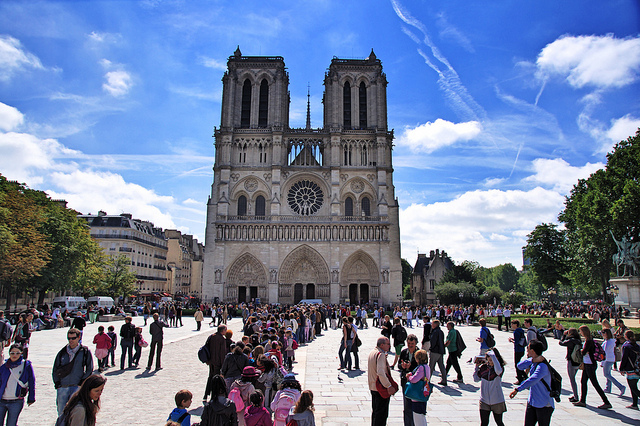
\includegraphics[width=8cm, height=6cm]{7498821028_6e7f113f4c_z_d.jpg}} 
		\hspace{20px}
		\fbox{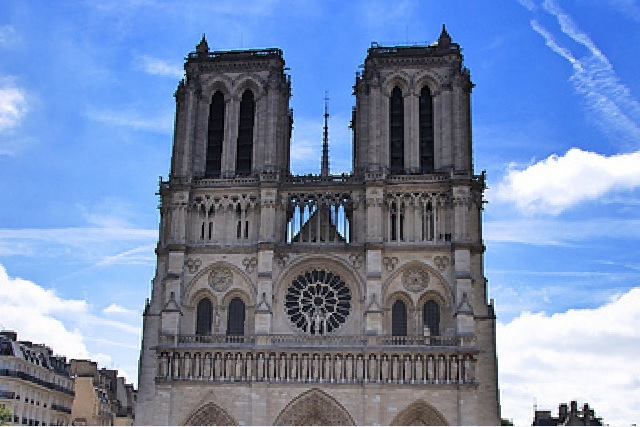
\includegraphics[width=8cm, height=6cm]{image2-warped.jpg}}
		\hspace{20px}
		\end{figure}
		
	\end{enumerate}
	
\textbf{How to run the code?} \newline

1.1) ./a2 part1.1 bigben\_2.jpg bigben\_3.jpg \newline

1.2) ./a2 part1.2 bigben\_2.jpg bigben\_3.jpg bigben\_6.jpg bigben\_7.jpg bigben\_8.jpg bigben\_10.jpg bigben\_14.jpg \newline

1.3) ./a2 part1.3 directory(/u/jagadiss/sagabhan-jagadiss-prakraja-a2/a2-images/part1\_images/) optional-src-image(/u/jagadiss/sagabhan-jagadiss-prakraja-a2/a2-images/part1\_images/eiffel\_18.jpg)\newline

1.4) ./a2 part1.4 directory(a2-images/part1\_images/) optional-src-img(bigben\_2.jpg)\newline

2.1) ./a2 part2 lincoln.png \newline

2.2) ./a2 part2 lincoln.png res.png \newline

2.3) ./a2 part2 lincoln.png f1.png f2.jpg  ..\newline

	
\end{document}

